\documentclass{article}
\usepackage[utf8]{inputenc}
\usepackage[english, swedish]{babel}
\usepackage{graphicx}
\usepackage{float}

\usepackage{lipsum}%% a garbage package you don't need except to create examples.

%For headers & footers
\usepackage{fancyhdr}
\pagestyle{fancy}
\lhead{
\includegraphics[scale=0.1516]{Logo}}
\chead{Kartrobot}
\rhead{2016-mm-dd}

\lfoot{Konstruktion med mikrodatorer}
\rfoot{Grupp 3 \\ ev. e-post till projektgrupp}

\renewcommand{\headrulewidth}{0.4pt}
\renewcommand{\footrulewidth}{0.4pt}


\title{Projektplan}
\author{Patrik Sletmo}
\date{September 2016}


\begin{document}
\graphicspath{{./images/}}
\selectlanguage{swedish}

\thispagestyle{empty}

{
\sffamily
\centering
\large


{\huge 
Projektplan
}

{\large
Patrik Sletmo
}

{\large
Version x.y
}

\vspace{13.5cm}

Status
\begin{center}
\begin{tabular}{ | c | c | c | } 
\hline
Granskad & snubbe & 2016-mm-dd \\
\hline
Godkänd & snubba & 2016-mm-dd\\
\hline
\end{tabular}
\end{center}
}

\clearpage

\topskip0pt
\vspace*{\fill}
{
\sffamily
\centering
\large


{\huge 
Projektidentitet
}

{\large
Grupp 3, 16/HT, KarToffel \\ Linköpings tekniska högskola, institution 
}

\vspace{0.5cm}

\begin{table}[H]
\centering
\begin{tabular}{ | c | c | c | c |} 
\hline
Namn & Ansvar & Telefon & E-post \\  
\hline
Patrik Sletmo & Projektledare & 070 783 57 61 & patsl736@student.liu.se \\
\hline
Rebecca Lindblom &  & 073 436 40 79 & rebli156@student.liu.se \\
\hline
Matildha Sjöstedt &  & 070 515 84 11 & matsj696@student.liu.se \\
\hline
Sebastian Callh &  & 073 820 46 64 & sebca553@student.liu.se \\
\hline
Anton Dalgren &  & 076 836 51 56 & antda685@student.liu.se \\
\hline
Matilda Dahlström &  & 070 636 33 52 & matda715@student.liu.se \\
\hline
\end{tabular}
\end{table}
}

\begin{center}
\textbf{Hemsida}: https://github.com/SebastianCallh/kartoffel-tsea29
\end{center}

\begin{center}
\textbf{Kund}: Mattias Krysander, 013 - 28 2198 , matkr@isy.liu.se
\end{center}

\begin{center}
\textbf{Kursansvarig}: Tomas Svensson, 3B 528, +46 (0)13 28 1368, tomas.svensson@liu.se \\
\textbf{Handledare}: Ännu ej bestämt
\end{center}
\vspace*{\fill}
\clearpage



\renewcommand*\contentsname{Innehållsförteckning}
\tableofcontents
\clearpage

\section{Beställare}
Beställare och köpare av projektet är Mattias Krysander, 013 - 28 2198, matkr@isy.liu.se

\section{Översiktlig beskrivning av projektet}

\subsection{Syfte och mål}
Syftet med det här projektet är att få förståelse för mikroprocessorer och kommunikationen mellan
dessa. Målet med detta projekt är att producera en robot som autonomt läser av ett rum och i realtid  ritar upp en karta över rummet.

\subsection{Leveranser}
Alla leveranser ska ske genom mail till beställaren i PDF-format, såvida inget annat står angivet. 

\begin{itemize}
    \item Kravspecifikationen ska vara godkänd senast den 2016-09-13. 
    \item Första versionen av projektplan, tidsplan och systemskiss ska vara inlämnad till beställaren senast 2016-09-22. 
    \item Slutgiltiga versionen av projektplan, tidsplan och systemskiss ska vara inlämnad till beställaren senast 2016-09-30. 
    \item Första versionen av designspecifikationen ska vara inlämnad till beställaren senast 2016-11-01. 
    \item Slutgiltiga versionen av designspecifikationen ska vara godkänd senast 2016-11-04.
    \item Efterstudien ska vara inlämnad senast 2016-12-21. 
    \item Utrustningen ska vara inlämnad senast 2016-12-22.
    \item Roboten ska levereras och redovisas senast vecka 51 till beställaren personligen.
    \item Teknisk dokumentation ska vara inlämnad senast tre arbetsdagar före redovisning.
    \item Användarhandledning ska vara inlämnad senast tre arbetsdagar före redovisning.
\end{itemize}


\subsection{Begränsningar}
Roboten ska ej förväntas fungera i en miljö utan tydliga konturer och hörn eller där det finns föremål som rör sig. Roboten förväntas heller inte fungera optimalt i ojämn terräng. Under projektet kommer ej någon omfattande utvärdering göras vad gäller vilka programmeringsspråk eller komponenter som är mest optimala.

\section{Fasplan}

\subsection{Före projektstart}
Innan projektets början ska en kravspecifikation tillsammans med projektplan, systemskiss och tidsplan färdigställas.

\subsubsection{Bilda projektgrupp}
En projektgrupp på sex studenter som läser kursen Konstruktion med mikrodatorer (TSEA29) ska bildas och rapporteras till kursens examinator. Samtidigt som gruppen bildas ska en projektledare utses.
   
\subsubsection{Kravspecifikation}
En kravspecifikation enligt LIPS-modellen ska skrivas och godkännas av projektets beställare, se leveranser.

\subsubsection{Ansvarsfördelning}
Alla roller förutom projektledaren ska bestämmas utifrån projektmedlemmarnas preferenser och erfarenheter. Rollerna ska ha en betydelse för tidsplanen.

\subsubsection{Tidsplan}
En tidsplan där alla projektmedlemmars tider planeras ska genomföras och godkännas av projektets beställare.

\subsubsection{Systemskiss}
En översiktlig beskrivning av systemet där det framgår hur produkten ska konstrueras ska skapas och godkännas av projektets beställare. Från skissen ska det gå att avgöra vilka moduler systemet innehåller och hur dess konstruktion kan delas in i arbetsblock.

\subsection{Under projektet}
Under projektet ska produkten designas, utvecklas och testas. Gruppen ska också tid- och statusrapportera.

\subsubsection{Design}
En designspecifikation ska tas fram och godkännas av handledaren och sedan lämnas till beställaren, se leveranser. 

\subsubsection{Utveckling}
Produktens alla delar ska konstrueras. Fysiska delar ska monteras ihop och mjukvara ska utvecklas.

\subsubsection{Tester}
Tester ska definieras och utföras på olika delar och nivåer av produkten för att säkerställa att produkten uppfyller kraven formulerade i kravspecifikationen.

\subsubsection{Planering}
Möten ska hållas och planering ska ske. Om så behövs redigeras en tidigare planering för att fungera under nya förutsättningar. Beslutsmöten ska hållas mellan projektgruppen och beställaren.

\subsubsection{Rapportering}
Tidrapportering ska skickas till beställaren veckovis under projektet. På beställarens begäran ska statusrapport skickas in.

\subsection{Efter projektet}
Efter projektet ska roboten presenteras inför beställare och kund, samt ingå i en tävling. En efterstudie ska också genomföras med syfte att utvärdera arbetet med projektet. Efter tävlingen ska roboten demonteras och alla komponenter återlämnas. Därmed finns ej någon avsikt att underhålla eller vidareutveckla roboten eller någon av delprodukterna. Projektgruppen kommer upplösas efter projektets slut.

\section{Organisationsplan för hela projektet}
``Allmän beskrivning av vad kapitlet innehåller''
\subsection{Organisationsplan per fas}

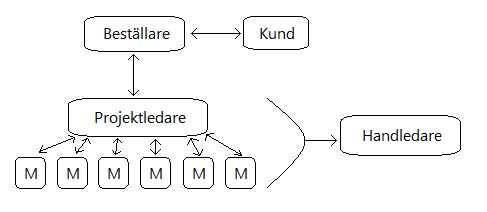
\includegraphics{Organisationsplan}
TODO:BILD

\subsection{Organisationsplan hos kunden}
Kunden och beställaren är samma person.

\subsection{Villkor för samarbetet inom projektgruppen}
\label{subsec:villkorsamarbete}

I slutet av varje vecka ska nästkommande veckas schema fastställas tillsammans med hela gruppen. Ifall man inte kan närvara på alla tillfällen som bestäms är det okej så länge man meddelar det i förväg. Även plötsliga orsaker till frånvaro är okej vid giltig frånvaro (t.ex. sjukdom, psykologiska problem, etc.).
\newline\newline
Till varje tillfälle som gruppen arbetar ska samtliga medlemmar komma väl förberedda. Har gruppen bestämt något som ska vara gjort till nästa gång ska varje gruppmedlem tagit på sig ansvaret att få det gjort i den mån det är möjligt.
\newline\newline
I början av varje vecka ska ett utvärderande möte hållas. Under det utvärderande mötet kan gruppens medlemmar lyfta fram åsikter om vad som fungerat bra respektive dåligt med projektet och samarbetet den senaste veckan. Det är okej att lyfta fram både positiv och negativ kritik så länge den framförs på ett professionellt sätt och kan argumenteras för. Kritik som uppkommer under veckans gång ska inte framföras förrän det utvärderande mötet om möjligt.
\newline\newline
Under arbetets gång ska arbetsuppgifterna fördelas likvärdigt i den mån det är möjligt. Eftersom det enligt beställarens direktiv ska avsättas exakt 160 timmar per person till projektet efter beslutspunkt 2 kommer alla medlemmar arbeta lika länge på projektet, även om det inte är synonymt med lika mycket. Gruppmedlemmar som inte har lagt sina 160 timmar riskerar att inte bli godkända enligt kursens upplägg.
\newline\newline
Alla gruppmedlemmar ska göra sitt bästa utan att överanstränga sig för att bidra till en kvalitativ leverans.
\newline\newline
Gruppen ska främst fokusera på fakta när beslut i gruppen tas. I de fall där någon gruppmedlem har tidigare erfarenhet av att ett annat alternativ fungerat bättre än det som stöds av fakta ska det övervägas och väljas ifall gruppmedlemmen kan framföra övertygande argument för sitt alternativ. Känslor ska inte tas hänsyn till för andra beslut än tidsplanering.

\subsection{Definition av arbetsinnehåll och ansvar}
\subsubsection{Projektledare}
Projektledaren ansvarar för att leda arbetet i gruppen framåt och är ansvarig utgivare för alla dokument gruppen producerar. Det är projektledarens uppgift att se till så att alla gruppmedlemmar arbetar utefter de riktlinjer som ställts i projektplanen. Projektledaren ansvarar också för att all kravställd dokumentation levereras till beställaren och att tidsrapportering för hela gruppen skickas in vid i förhand bestämda tillfällen. Utöver projektledaransvaret är projektledaren även utvecklare till 90\%.

\section{Dokumentplan}


\section{Utvecklingsmetodik}

\section{Utbildningsplan}
Projektmedlemmarna får som förberedelse till projektet delta i sex stycken föreläsningar samt en labb i Mätteknik som ges i kursen Konstruktion med Mikrodatorer (TSEA29). Labben ska låta utbilda projektdeltagarna i att använda en logikanalysator. Kunden behöver ej genomgå någon särskild utbildning för att förstå projektets interna eller externa struktur.

\section{Rapporteringsplan}
En tidsrapport ska levereras till beställaren veckovis varje måndag senast kl 16:00 från och med 31/10 till och med 19/12. Leveransen ska ske från projektledaren, är projektledaren frånvarande ska första närvarande gruppmedlem enligt ordningen i tabellen på sida två i kravspecifikationen genomföra leveransen.

\section{Mötesplan}
De enda officiella mötena sker på måndagar i form av utvärderingsmöten, se avsnitt~\ref{subsec:villkorsamarbete}. Alla utvärderingsmöten antecknas och läggs upp på gruppens gemensamma mapp på Google Drive. Ifall ett extra möte krävs kan en gruppmedlem utlysa detta på Slack.

\section{Resursplan}
Detta avsnitt innehåller information om resurser inom projektet.
\subsection{Personer}
Gruppen består utav 6 personer som totalt ska arbeta 960 timmar med projektet efter beslutspunkt 2.
\begin{itemize}
  \item Patrik Sletmo
  \item Sebastian Callh
  \item Matilda Dahlström
  \item Anton Dalgren
  \item Rebecca Lindblom
  \item Matildha Sjöstedt
\end{itemize}
Alla i gruppen ska jobba lika mycket d.v.s. 160 timmar var efter beslutspunkt 2.
\newline\newline
Som resurs finns även en handledare att anlita vid behov. Om handledaren anser det nödvändigt hänvisar den till en teknisk expert inom det efterfrågade området. 
\subsection{Material}
Projektet kräver flertalet komponenter och mätutrustning. All utrustning finns tillhandahållen av universitetet och behöver inte beställas. Projektet kommer kräva elektronikkomponenter, t.ex. processorer, sensorer och servon. Det kommer även att krävas en laptop med Bluetooth. Projektmedlemmarna behöver ha tillgång till varsin dator med tillhörande programvaror för utveckling.   
\subsection{Lokaler}
Till projektets förfogande finns lokalerna Muxen 3-4 där dator och mätutrustning för hårdvaruutveckling finns att tillgå. Dessa lokaler är alltid tillgängliga efter beslutpunkt 2 och alla i gruppen kan vara där samtidigt. Vid eventuell platsbrist i Muxen kan gruppen hitta andra lediga ytor att arbeta på. Om det skulle ske så tas ett beslut inom gruppen om vilka medlemmar som behöver stanna kvar i Muxen.
\subsection{Ekonomi}
Projektet har en budget på max 160 arbetstimmar per person efter att beslutpunkt 2 har tagits.

\section{Milstolpar och beslutspunkter}
\subsection{Milstolpar}
\begin{center}
  \begin{tabular}{ | l | l | l | }
    \hline
    1 & Kravspecifikation klar & 2016-09-08 \\ \hline
    2 & Projektplan, tidsplan och systemskiss klar & 2016-09-23  \\ \hline
    3 & Designspecifikation klar & 2016-10-29 \\ \hline
    4 & Robot kan fjärrstyras (???) & 2016-11-20 \\ \hline
    n &  &  \\ 
    \hline
  \end{tabular}
\end{center}
\subsection{Beslutspunkter}
\begin{center}
  \begin{tabular}{ | l | l | l | }
    \hline
    0 & Godkännande av projektdirektiv, beslut att starta förstudie & 2016-09-01 \\ \hline
    1 & Godkännande av kravspecifikation, beslut att starta förberedelsefasen & 2016-09-13 \\ \hline
    2 & Godkännande av projektplanen, beslut att starta utförandefasen & 2016-09-29 \\ \hline
    3 & Godkännande av designspecifikationen, beslut att fortsätta uförandefasen & 2016-11-01 \\ \hline
    4 & Används ej &  \\ \hline
    5 & Godkännande av produktens funktionalitet, beslut att leverera & 2016-12-15 \\ \hline
    6 & Godkännande av leverans, beslut att upplösa projektgruppen & XXXX-YY-ZZ \\
    \hline
  \end{tabular}
\end{center}

\section{Aktiviteter}
\section{Tidplan}
\section{Förändringsplan}
Utifall att krav specificerade i kravspecifikationen ej kan uppnås eller tvingas omprioriteras, pga. till exempel tekniska problem eller tidsbrist, måste de nya kraven godkännas av beställaren. Vid större förseningar som resulterar i att robotens grundläggande krav inte kan uppfyllas innan projektets avslut (se Projektavslut) blir konsekvensen att projektet ej blir godkänt.  

\section{Kvalitetsplan}

\subsection{Granskningar}
\subsection{Testplan}

\section{Riskanalys}
\section{Prioriteringar}
\section{Projektavslut} 
Projektet avslutas genom en presentation (v 51, år 2016) inför beställare och kund samt en tävling enligt dokumentet \textit{Ban- och tävlingsspecifikation för kartrobotar 2016}, där andra robotar med samma funktionsmål deltar. Presentationen syfte är att t.ex. lyfta fram särskilda tekniska lösningar och "göra reklam" för vår grupp inför beställaren. All utlånad utrustning - inklusive robotens komponenter - ska återlämnas senast den 22/12 till handledaren. Projektet ska efter sitt slut utvärderas i en efterstudie. Här kommer ska bl.a. samarbetet i projektgruppen, relation med beställare och handledare samt tekniska problem diskuteras. Projektdeltagarna ska inte göra någon individuell uppföljning vad gäller sina färdigheter i projektarbete. 

\end{document}
